Using SI units, the given parameters are
\[
L=0.568\ \mathrm{m},\quad m=5.35\ \mathrm{kg},\quad
E=200\times10^{9}\ \mathrm{Pa},\quad
h=0.003\ \mathrm{m},\quad b=0.037\ \mathrm{m},
\]
\[
g=9.81\ \mathrm{m/s^2},\qquad Y=710\times10^{6}\ \mathrm{Pa}.
\]
The mass is attached at the undeformed tip and is initially at rest.

\[
\boxed{\begin{gathered}
L=0.568\ \mathrm{m},\quad m=5.35\ \mathrm{kg},\quad E=200\ \mathrm{GPa},\\
h=3\ \mathrm{mm},\quad b=37\ \mathrm{mm},\quad
g=9.81\ \mathrm{m/s^2},\quad Y=710\ \mathrm{MPa}
\end{gathered}}
\qquad\text{(C.6.1)}
\]

The beam bends vertically, so the cross-section dimension \(h\) lies in the bending direction. For the rectangular cross-section, the second moment of area is
\[
I=\frac{bh^3}{12}
 =\frac{(0.037)(0.003)^3}{12}
 =8.325\times10^{-11}\ \mathrm{m^4}
 =83.25\ \mathrm{mm^4}.
\]
The flexural rigidity is then
\[
EI=(200\times10^9)(8.325\times10^{-11})
 =16.65\ \mathrm{N\,m^2}.
\]

For a cantilever with a concentrated tip load, the end displacement is \(\Delta=PL^3/(3EI)\). Therefore, the equivalent spring constant is
\[
k=\frac{P}{\Delta}=\frac{3EI}{L^3}
 =\frac{3(16.65)}{(0.568)^3}
 =272.5778\ \mathrm{N/m}.
\]
The natural frequency and period follow from
\[
\omega_n=\sqrt{\frac{k}{m}}
 =\sqrt{\frac{272.5778}{5.35}}
 =7.1379\ \mathrm{rad/s},
\]
\[
f_n=\frac{\omega_n}{2\pi}=1.1360\ \mathrm{Hz},
\qquad
\tau=\frac{2\pi}{\omega_n}=0.88026\ \mathrm{s}.
\]

\[
\boxed{\begin{aligned}
I&=83.25\ \mathrm{mm^4},&
EI&=16.65\ \mathrm{N\,m^2},&
k&=272.58\ \mathrm{N/m},\\
\omega_n&=7.138\ \mathrm{rad/s},&
f_n&=1.136\ \mathrm{Hz},&
\tau&=0.8803\ \mathrm{s}
\end{aligned}}
\qquad\text{(C.6.2)}
\]

The applied weight is
\[
F_0=mg=(5.35)(9.81)=52.4835\ \mathrm{N}.
\]

\[
\boxed{F_0=52.48\ \mathrm{N}}\qquad\text{(C.6.3)}
\]

For the gradual-release case, the mass reaches equilibrium without oscillating. Setting the acceleration to zero gives
\[
ku_{\mathrm{st}}=F_0,
\qquad
u_{\mathrm{st}}=\frac{F_0}{k}
 =\frac{52.4835}{272.5778}
 =0.192545\ \mathrm{m}.
\]
Thus, the static tip displacement is \(192.545\ \mathrm{mm}\).

\[
\boxed{u_{\mathrm{st}}=192.55\ \mathrm{mm}}\qquad\text{(C.6.4)}
\]

For the sudden-release case, the load is applied at \(t=0\) while the mass is still at the undeformed position. The equation of motion for \(t>0\) is
\[
m\ddot u+ku=F_0.
\]
The at-rest initial conditions are
\[
u(0)=0,\qquad \dot u(0)=0.
\]
Using the constant particular solution \(u_p=F_0/k\) and the complementary solution \(u_c=A\cos(\omega_nt)+B\sin(\omega_nt)\), these initial conditions give \(A=-F_0/k\) and \(B=0\). Therefore, the displacement measured from the undeformed position is
\[
u(t)=\frac{F_0}{k}\left[1-\cos(\omega_nt)\right]
 =0.192545\left[1-\cos(7.1379t)\right]\ \mathrm{m}.
\]

The largest value occurs when \(\cos(\omega_nt)=-1\), which first occurs at
\[
t_{\max}=\frac{\pi}{\omega_n}=0.44013\ \mathrm{s}.
\]
Consequently,
\[
u_{\mathrm{dyn}}=u_{\max}
 =\frac{2F_0}{k}
 =2u_{\mathrm{st}}
 =0.385090\ \mathrm{m}.
\]
In millimetres, this is \(385.090\ \mathrm{mm}\).

\[
\boxed{u_{\mathrm{dyn}}=u_{\max}=385.09\ \mathrm{mm}
\quad\text{at}\quad t_{\max}=0.4401\ \mathrm{s}}
\qquad\text{(C.6.5.a)}
\]

For \(N_{\mathrm{osc}}=10\), the plotting interval is
\[
t_{\mathrm{end}}=N_{\mathrm{osc}}\tau
 =10(0.88026)
 =8.8026\ \mathrm{s}.
\]
The response plot below is measured from the undeformed beam position. The dashed line is the static displacement, and the square marker identifies the first dynamic maximum.

\begin{figure}[H]
\centering
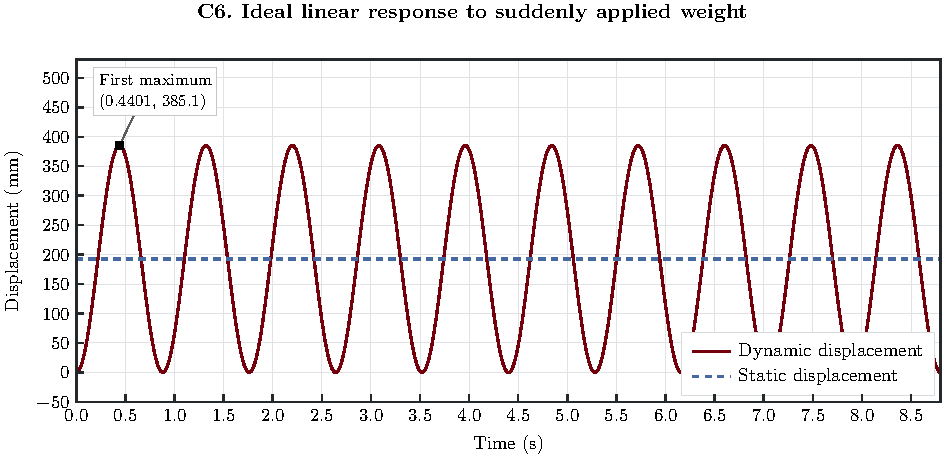
\includegraphics[width=0.95\linewidth,height=0.30\textheight,keepaspectratio,alt={C.6. Ideal linear response to suddenly applied weight over ten oscillations, with the first maximum marked.}]{figures/generated/solutions/C6.pdf}
\caption{C.6. Ten-cycle response measured from the undeformed position.}
\end{figure}

\[
\boxed{N_{\mathrm{osc}}=10,\qquad t_{\mathrm{end}}=8.8026\ \mathrm{s}}
\qquad\text{(C.6.5.b)}
\]

The data tip at the first maximum reads approximately
\[
(t_{\max},u_{\max})=(0.440\ \mathrm{s},385\ \mathrm{mm}).
\]
This agrees with the analytical value in item (5)(a) to the precision shown.

\[
\boxed{u_{\mathrm{tip}}(0.440\ \mathrm{s})=385\ \mathrm{mm}
\approx u_{\mathrm{dyn}}}
\qquad\text{(C.6.5.c)}
\]

\matlabcaption{C.6 response plot.}
\begin{matlabcode}
L=.568; E=200e9; h=.003; b=.037; m=5.35; g=9.81;
Nosc=10; I=b*h^3/12; k=3*E*I/L^3; wn=sqrt(k/m);
F0=m*g; ust=F0/k; tau=2*pi/wn;
t=linspace(0,Nosc*tau,2000); u=ust*(1-cos(wn*t));
tmax=pi/wn; umax=2*ust;
plot(t,1000*u,'Color',[0 .427 .459],'LineWidth',1.5);
hold on; plot(t,1000*(ust+0*t),'--','Color',[.776 .365 0],'LineWidth',1.2);
plot(tmax,1000*umax,'ks'); grid on;
xlabel('Time (s)'); ylabel('Displacement (mm)');
\end{matlabcode}

\par\addvspace{0.35em}
For the static case, the root bending moment is the applied weight multiplied by the beam length,
\[
M_{\mathrm{st}}=F_0L=(52.4835)(0.568)=29.8106\ \mathrm{N\,m}.
\]
The outer-fibre distance is \(c=h/2=0.0015\ \mathrm{m}\). Using the flexure relation \(\sigma=Mc/I\), the static root stress is
\[
\sigma_{\mathrm{st}}
 =\frac{M_{\mathrm{st}}c}{I}
 =\frac{(29.8106)(0.0015)}{8.325\times10^{-11}}
 =5.3713\times10^8\ \mathrm{Pa}
 =537.13\ \mathrm{MPa}.
\]
The corresponding safety factor is
\[
\mathrm{SF}_{\mathrm{st}}
 =\frac{Y}{\sigma_{\mathrm{st}}}
 =\frac{710}{537.13}
 =1.322.
\]

\[
\boxed{\sigma_{\mathrm{st}}=537.13\ \mathrm{MPa},\qquad
\mathrm{SF}_{\mathrm{st}}=1.322}
\qquad\text{(C.6.6.a)}
\]

At the dynamic maximum, the beam restoring force is
\[
P_{\mathrm{dyn}}=ku_{\mathrm{dyn}}=2F_0.
\]
Therefore, the dynamic root moment is twice the static root moment,
\[
M_{\mathrm{dyn}}=P_{\mathrm{dyn}}L=2F_0L=59.6213\ \mathrm{N\,m}.
\]
The maximum dynamic stress and its safety factor are
\[
\sigma_{\mathrm{dyn}}
 =\frac{M_{\mathrm{dyn}}c}{I}
 =1.0743\times10^9\ \mathrm{Pa}
 =1074.26\ \mathrm{MPa},
\]
\[
\mathrm{SF}_{\mathrm{dyn}}
 =\frac{Y}{\sigma_{\mathrm{dyn}}}
 =\frac{710}{1074.26}
 =0.661.
\]

\[
\boxed{\sigma_{\mathrm{dyn}}=1074.26\ \mathrm{MPa},\qquad
\mathrm{SF}_{\mathrm{dyn}}=0.661}
\qquad\text{(C.6.6.b)}
\]

The static safety factor is slightly greater than one, so the ideal static calculation remains below the specified yield stress. The sudden release doubles the tip displacement, root moment, and bending stress, which reduces the safety factor below one. The linear model therefore predicts yielding in the dynamic case. The predicted dynamic displacement is also \(0.678L\), so large-deflection geometry and material nonlinearity would become important before the ideal linear response could be realized.

\[
\boxed{\mathrm{SF}_{\mathrm{dyn}}<1\ \Rightarrow\ \text{yielding is predicted in the dynamic case}}
\qquad\text{(C.6.7)}
\]
